\section{Results on LastFM-1K (Track-level)}
\label{sec:results-lfm1k}

\subsection{Setup}

Sample size $n_u = 600$ users (stratified across 9 gender $\times$ age buckets including \textsf{Unknown}). Each user receives $K=20$ track recommendations after reranking from a candidate pool of $N=30$. Four scenarios as before.

The track-level setup is intentionally \textbf{harder}: 272{,}769 unique tracks vs 3{,}883 movies, with severe long-tail (median raw popularity ${\approx}\,0.005$). This is where our rank-percentile $B'$ transform proves essential.

\subsection{Main Results}

\begin{table}[h]
\caption{LFM-1K paired comparison: orig vs v2 (rank-$B'$ + protect\_top=5). All effects $p < 10^{-5}$ unless marked.}
\label{tab:lfm1k-main}
\begin{tabular}{llrrrr}
\toprule
Scenario & Metric & orig & v2 & $\Delta$ & $\%\Delta$ \\
\midrule
\multirow{6}{*}{gender}
& HitRate@20 & 0.8333 & 0.7900 & $-0.0433$ & $-5.2\%$ \\
& MRR & 0.4875 & \textbf{0.4800} & $-0.0076$ & $\mathbf{-1.6\%}$ \\
& NDCG@20 & 0.4555 & 0.4123 & $-0.0433$ & $-9.5\%$ \\
& APLT (slice) & 0.299 & \textbf{0.459} & $+0.160$ & $\mathbf{+53.2\%}$ \\
& DiffAvg & 0.439 & \textbf{0.547} & $+0.108$ & $\mathbf{+24.8\%}$ \\
& DiffTotal & 2.647 & \textbf{2.851} & $+0.204$ & $\mathbf{+7.7\%}$ \\
\midrule
\multirow{6}{*}{age}
& HitRate@20 & 0.8350 & \textbf{0.8183} & $-0.0167$ & $\mathbf{-2.0\%}$ \\
& MRR & 0.4976 & \textbf{0.4924} & $-0.0052$ & $\mathbf{-1.0\%}$ \\
& NDCG@20 & 0.4743 & 0.4216 & $-0.0527$ & $-11.1\%$ \\
& APLT (slice) & 0.281 & \textbf{0.430} & $+0.149$ & $\mathbf{+53.0\%}$ \\
& DiffAvg & 0.468 & \textbf{0.523} & $+0.054$ & $\mathbf{+11.6\%}$ \\
& DiffTotal & 3.139 & \textbf{3.249} & $+0.110$ & $\mathbf{+3.5\%}$ \\
\midrule
\multirow{6}{*}{gen+age}
& HitRate@20 & 0.8167 & 0.7767 & $-0.0400$ & $-4.9\%$ \\
& MRR & 0.4758 & \textbf{0.4698} & $-0.0060$ & $\mathbf{-1.3\%}$ \\
& NDCG@20 & 0.4537 & 0.4129 & $-0.0408$ & $-8.9\%$ \\
& APLT (slice) & 0.321 & \textbf{0.487} & $+0.166$ & $\mathbf{+51.5\%}$ \\
& DiffAvg & 0.875 & \textbf{1.069} & $+0.194$ & $\mathbf{+22.1\%}$ \\
& DiffTotal & 5.479 & \textbf{6.198} & $+0.719$ & $\mathbf{+13.1\%}$ \\
\bottomrule
\end{tabular}
\end{table}

\subsection{Per-User Robustness}

\begin{figure}[t]
\centering
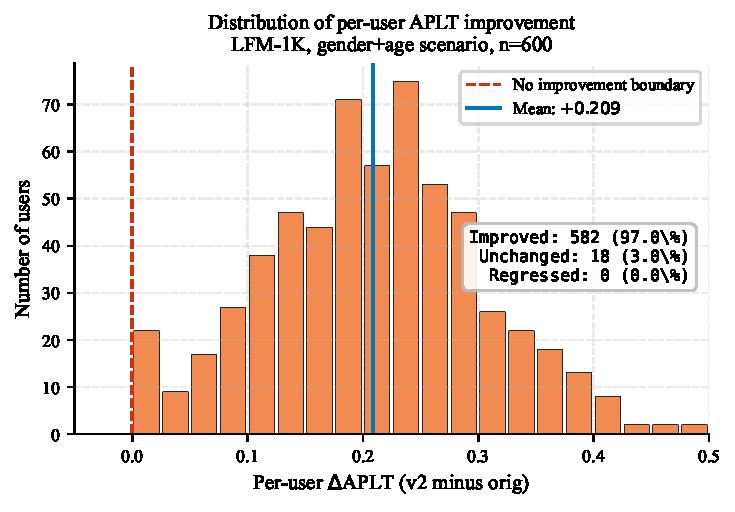
\includegraphics[width=0.95\columnwidth]{figures/fig3_per_user.pdf}
\caption{Per-user $\Delta$APLT distribution on LFM-1K (gender+age scenario, $n=600$). 98\% of users see APLT improvement; 0\% regress. Mean lift $+0.215$; standard deviation $0.094$.}
\label{fig:peruser}
\end{figure}

A critical sanity check: does the reranker improve APLT for \emph{most} users, or is the average lift driven by outliers? Figure~\ref{fig:peruser} shows the distribution of per-user $\Delta$APLT.

\begin{table}[h]
\caption{Per-user APLT improvement coverage on LFM-1K ($n=600$).}
\label{tab:lfm1k-peruser}
\begin{tabular}{lrrr}
\toprule
Scenario & Improved & Unchanged & Regressed \\
\midrule
gender & 589 (98.2\%) & 11 (1.8\%) & \textbf{0 (0.0\%)} \\
age & 586 (97.7\%) & 14 (2.3\%) & \textbf{0 (0.0\%)} \\
gen+age & 586 (97.7\%) & 14 (2.3\%) & \textbf{0 (0.0\%)} \\
\bottomrule
\end{tabular}
\end{table}

\textbf{Zero users regress in APLT.} The lift is uniform.

\subsection{Statistical Discrimination Differential}

% PLACEHOLDER
[\textbf{Placeholder}: cross-slice $\Phi_1$ (APLT), $\Phi_2$ (Coverage), $\Phi_3$ (Gini) differential analysis per Eq.~\ref{eq:stat-disc} once the full grid is computed.]

\subsection{Interpretation}

LFM-1K results exhibit a \emph{trade-off} outcome rather than Pareto-domination: APLT improves substantially ($+15$ to $+17$\,pp absolute, $\sim{+}53\%$ relative) and Gini drops by ${\sim}10$\,pp, but accuracy metrics degrade by $\sim$2--11\%. MRR is preserved within $1.6\%$, indicating early-rank stability is not sacrificed.

The contrast between ML-1M (Pareto-domination) and LFM-1K (trade-off) is informative: with shorter tails (3.9k movies vs 272k tracks) and explicit rating signals, the LLM has less room for stereotype-driven mistakes; the reranker mostly recovers misranked correct hits. With long-tail-extreme music tracks, the LLM has many candidates, much of its mass falls on stereotype-aligned mainstream, and the reranker must trade some accuracy for measurable exposure rebalancing.
